\documentclass[a4paper]{article}

\usepackage{graphicx}
\usepackage{amsmath,amssymb}
\usepackage{minted}
\usepackage{multirow}
\usepackage{float}
\usepackage{todonotes}
\usepackage{forest}
\usepackage{xstring}
\usepackage{xcolor}
\usepackage[most]{tcolorbox}
\usepackage{xparse}
\usepackage{natbib}

\usetikzlibrary{graphs,graphdrawing}
\usegdlibrary{layered}

% for external graphviz
\input{/home/donkarlo/Dropbox/repo/nd_ai_project/src/nd_ai/knoweldge_representation/language/formal/computer/programming/tex/latex/code_clips/external_graphviz.tex}

% for tags
\input{/home/donkarlo/Dropbox/repo/nd_ai_project/src/nd_ai/knoweldge_representation/language/formal/computer/programming/tex/latex/parts/control_sequence/kind/semtag/semtag.tex}

% for links
\input{/home/donkarlo/Dropbox/repo/nd_ai_project/src/nd_ai/knoweldge_representation/language/formal/computer/programming/tex/latex/code_clips/seehere.tex}

\title{Aerial Orthophotos}
\date{}
\author{Mohammad Rahmani}

\begin{document}
    \maketitle
    
    
    \section{Aerial Orthophotos (Aerial orthophotos (high-resolution, top-down))}
        An orthophoto, orthophotograph, orthoimage or orthoimagery is an aerial photograph or satellite imagery geometrically corrected ("orthorectified") such that the scale is uniform: the photo or image follows a given map projection. Unlike an uncorrected aerial photograph, an orthophoto can be used to measure true distances, because it is an accurate representation of the Earth's surface, having been adjusted for topographic relief,[1] lens distortion, and camera tilt \seeherefooter{https://en.wikipedia.org/wiki/Orthophoto}.
    
        Aerial orthophotos are geometrically corrected top-down images in which scale is approximately uniform across the scene.
        Their high spatial resolution makes roof boundaries, roof-mounted equipment, vegetation, and many surface differences visible at building level.
        Because the images are rectified, they can be aligned directly with cadastral parcels or building-footprint polygons and used for area measurement.
        Their main limitations are acquisition date, shadows, seasonal vegetation, residual displacement around tall objects, and incomplete information about roof slope.
        For Vienna, official orthophoto access is available through the city mapping services \seeherefooter{https://www.wien.gv.at/stadtplanung/orthofoto-stadtplansuche} and the Austrian open-data portal \seeherefooter{https://www.data.gv.at/}.
        
        \begin{figure}[H]
            \centering
            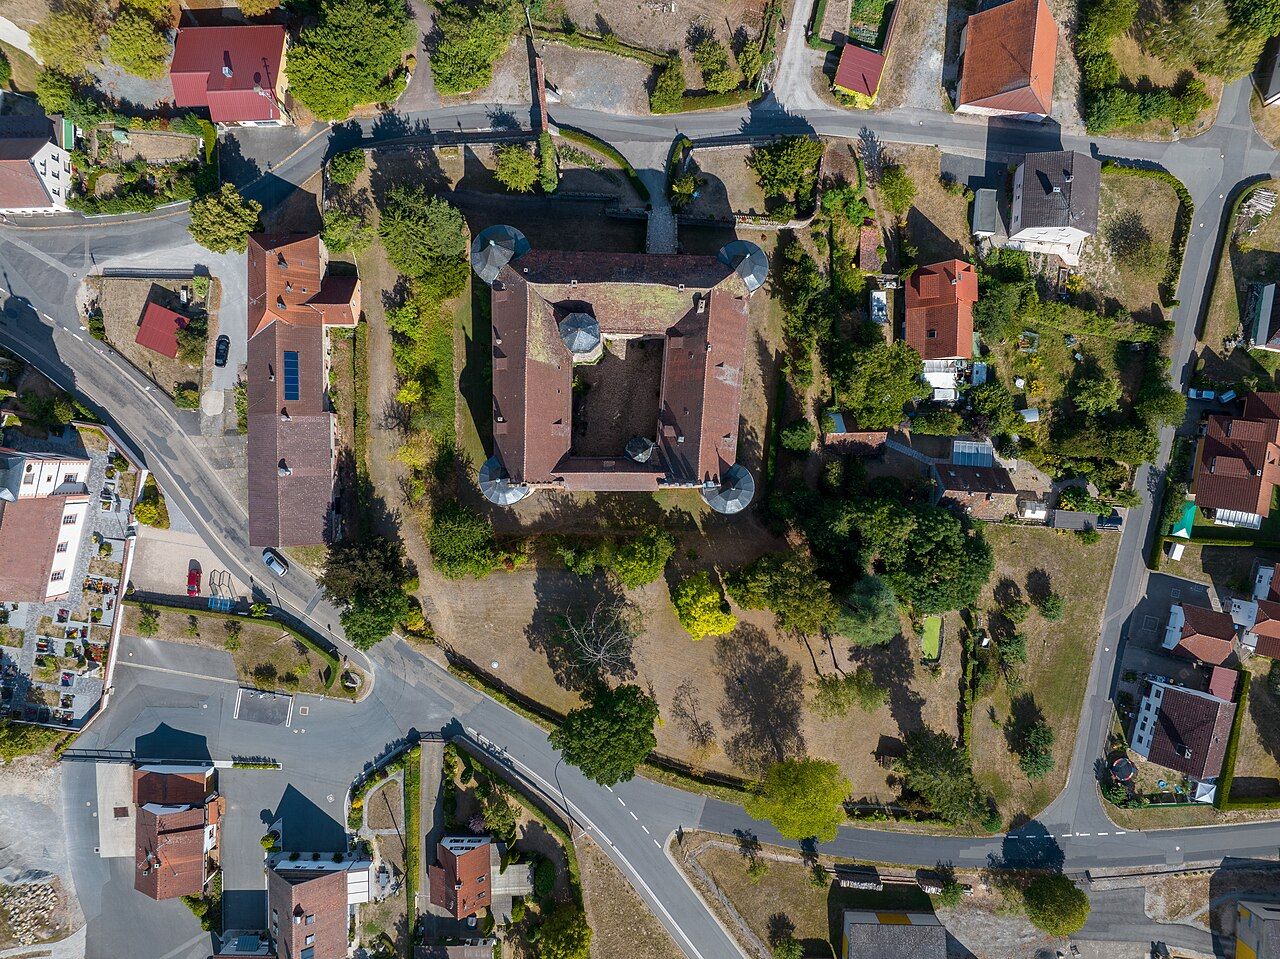
\includegraphics[width=0.82\textwidth]{images/aerial_orthophotos_example.jpg}
            \caption{Example of a true orthophoto with a near-vertical, geometrically corrected view.}
        \end{figure}
        \noindent\small Image source and licence information: \seeherefooter{https://commons.wikimedia.org/w/index.php?oldid=1162345206}.\normalsize
        
%        \bibliographystyle{plainnat}
%        \bibliography{/home/donkarlo/Dropbox/repo/nd_shared_research/bibliography/bibliography.bib}
\end{document}
